\renewcommand{\theequation}{\theenumi}
\begin{enumerate}[label=\arabic*.,ref=\thesubsection.\theenumi]
\numberwithin{equation}{enumi}
\item From the gernelised form of the eqautions 
\begin{align}
minZ &= c^t \vec{x}
\\
\text{subjected to}
\\
A\vec{x} &\preceq b
\\ 
\text{we can find $\to$ }
\\
c &= \myvec{200\\ 500}
\\
A &= \myvec{-1 & -2 \\ 3 & 4}
\\
b &= \myvec{-10\\ 24}
\\
\end{align}\\
Solution for the above equations can be find from the python code of Lenear programing 
\begin{lstlisting}
./optimization/codes
\end{lstlisting}
From the codes we get that the minimum value of the equation will be 2299.99 at the point $\myvec{4 & 3}$.

\begin{figure}[!ht]
	\centering
	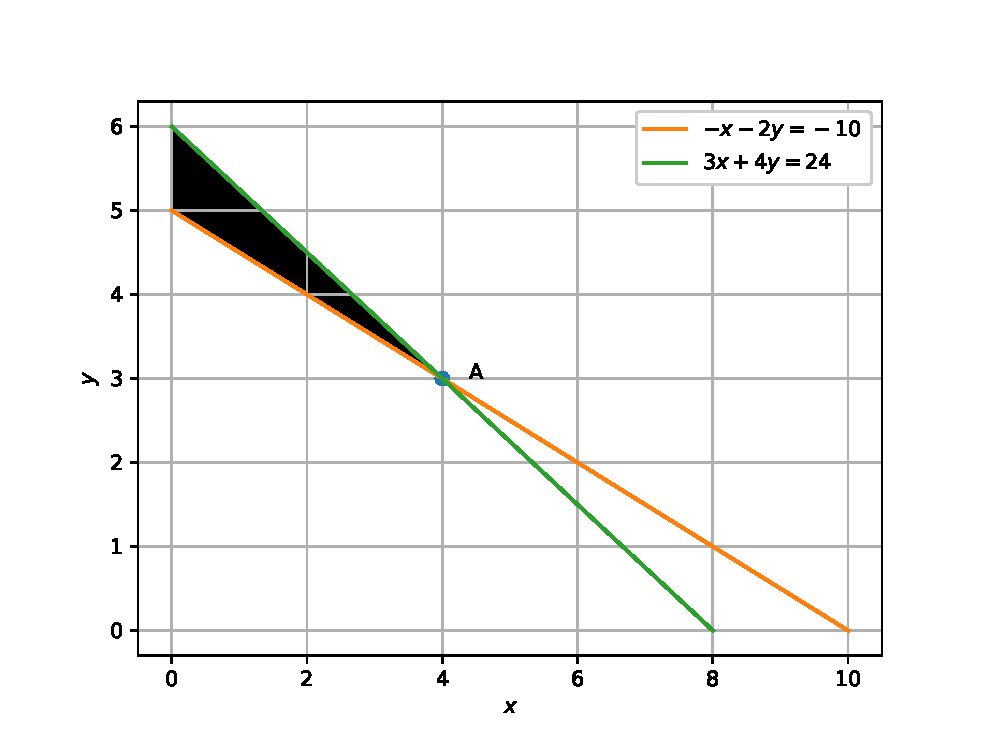
\includegraphics[width=\columnwidth]{./figures/lp2.eps}
	\caption{ lp2 }
	\label{fig:lp2}
	Pythone codes for the above figure can be get from
	\begin{lstlisting}
	./optimization/figures/lp2.eps
	\end{lstlisting}	
\end{figure}
\end{enumerate}